\subsubsubsubsection{District starter}
\begin{figure}[h]
\centering
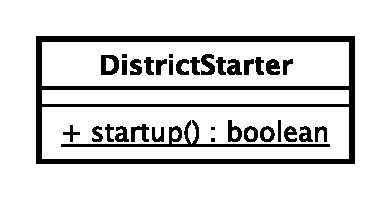
\includegraphics[scale=0.6,keepaspectratio]{images/solution/app/backend/district_starter.eps}
\caption{\pReactive::DistrictStarter}
\label{fig:sd-app-district-starter}
\end{figure}
\FloatBarrier
\begin{itemize}
  \item \textbf{\descr} \\
  It has the responsibility to boot the application layer.
  \item \textbf{\ops}
  \begin{itemize}
    \item[+] \texttt{\underline{startup() : boolean}} \\
    Boots the application layer running all the active entities of the 
    district (urban actors and traffic lights).
    Returns true if the process completes neatly, false otherwise.
  \end{itemize}
\end{itemize} 
